%% BMC Bioinformatics submission -- built against the official bmcart class.
\documentclass{bmcart}

\usepackage{amsthm,amsmath}
\usepackage[utf8]{inputenc}
\usepackage{graphicx}
\usepackage{url}

\startlocaldefs
\endlocaldefs

\begin{document}

\begin{frontmatter}

\begin{fmbox}
\dochead{Research}

\title{Leakage-Free Evaluation of Single-Cell Treatment Response Classifiers Reveals Systematic Underpowering in Small Public Cohorts}

\author[
  addressref={aff1},
  corref={aff1},
  email={patrickchoi@usf.edu}
]{\inits{P.}\fnm{Patrick} \snm{Choi}}

\address[id=aff1]{%
  \orgdiv{Department of Integrative Biology},
  \orgname{University of South Florida},
  \city{Tampa},
  \state{FL},
  \cny{USA}
}

\end{fmbox}

\begin{abstractbox}

\begin{abstract}
\parttitle{Background}
Machine learning frameworks using single-cell RNA sequencing data are increasingly applied to predict treatment response and identify biomarker signatures. However, a pervasive methodological flaw, performing highly variable gene selection and feature scaling globally across all cells prior to cross-validation splits, introduces systematic data leakage. In clinical cohorts with small sample sizes, this leakage artificially inflates model performance, leading to over-optimistic results that fail to generalize and presenting a significant challenge to reproducible marker discovery.

\parttitle{Methods}
We applied a leakage-free nested Leave-One-Out Cross-Validation framework to two independent single-cell datasets: an inflammatory bowel disease anti-TNF cohort ($n=36$) and a melanoma immune checkpoint inhibitor cohort ($n=18$ baseline patients). Feature selection using ANOVA ($k=5$) and scaling were embedded strictly within each training fold. Statistical significance was evaluated using a 500-iteration nested permutation test. External bulk validation was performed on baseline melanoma patients from GSE91061 ($n=33$).

\parttitle{Results}
Both classifiers achieved approximately 72\% nominal accuracy with moderate area under the curve values (IBD: 0.766, melanoma: 0.741). After leak correction, neither model survived nested permutation testing (IBD $p=0.0878$, melanoma $p=0.2056$). Consensus signatures emerged, featuring \textit{TNK1} (100\% of IBD folds) and \textit{TBC1D10B} (100\%) and \textit{TNRC6B} (94.4\%) in melanoma. External bulk validation confirmed that no individual signature gene reached significance (0/6, $p < 0.05$); 83.3\% showed the expected direction, though not significantly (two-sided binomial $p = 0.219$).

\parttitle{Conclusions}
Current public single-cell treatment response cohorts are systematically underpowered. Global preprocessing before cross-validation splits inflates significance, making properly nested permutation architectures mandatory for biomarker validation. The most stable biological signals identified in this study, notably \textit{TNK1}, warrant targeted validation in larger prospective patient cohorts.
\end{abstract}

\begin{keyword}
\kwd{single-cell RNA sequencing}
\kwd{data leakage}
\kwd{nested cross-validation}
\kwd{inflammatory bowel disease}
\kwd{anti-TNF therapy}
\kwd{immune checkpoint inhibitor}
\kwd{biomarker discovery}
\kwd{permutation testing}
\end{keyword}

\end{abstractbox}

\end{frontmatter}

\section*{Background}
The clinical utility of precision medicine in chronic inflammatory and oncological conditions relies on baseline stratification of patient response profiles. In IBD, anti-tumor necrosis factor (anti-TNF) monoclonal antibodies such as adalimumab are frontline interventions, yet 30\% to 40\% of patients experience therapeutic failure \cite{roda}. Similarly, immune checkpoint inhibitors (ICIs) have revolutionized oncology, but most patients with metastatic melanoma fail to achieve durable remission. In both contexts, exposing non-responding patients to ineffective therapies causes avoidable toxicity, increases healthcare costs, and delays clinical access to alternative therapeutic options \cite{alatab,roda}. Consequently, identifying baseline predictive biomarkers is a critical clinical objective to guide therapeutic selection and optimize patient outcomes \cite{alatab,riaz,sadefeldman}.

To address this need, machine learning (ML) frameworks using single-cell RNA sequencing (scRNA-seq) data have grown rapidly to resolve cell-type-specific transcriptional signatures of treatment response. For example, the PRECISE framework demonstrated the utility of interpretable single-cell classifiers for predicting immunotherapy response across multiple cancer types \cite{pinhasi}. Prior transcriptomic studies have identified disease-relevant programs such as the GIMATS module in anti-TNF-resistant Crohn's disease \cite{martin} and specific T-cell exhaustion states in melanoma ICI response \cite{sadefeldman}. Consistent with this, Friedrich and colleagues combined bulk and single-cell transcriptomics across multiple IBD cohorts to define an inflammatory pathotype, marked by neutrophil infiltration, fibroblast activation, and vascular remodeling, that characterizes a subset of patients who do not respond to current therapies \cite{friedrich}. Building on these findings, ML frameworks have emerged to translate such programs into patient-level response classifiers. By integrating compositional features and pseudo-bulk transcriptional expressions, these models aim to capture multi-layered biological signals. However, translating these classifiers into clinical diagnostics requires rigorous statistical validation.

Despite their promise, single-cell ML pipelines are vulnerable to systematic data leakage. The consequences of leakage for genomic machine learning are well documented in general terms: preprocessing operations such as feature scaling and supervised feature selection, when applied across all samples before cross-validation, yield optimistically biased performance estimates \cite{whalen}, and leakage has been identified as a recurrent driver of irreproducible ML-based science across disciplines \cite{kapoor}. A closely related hazard, pseudoreplication, is well established in single-cell differential expression, where treating individual cells as independent observations inflates statistical confidence because cells from the same patient are not independent \cite{squair}. The unifying principle in both cases is that the patient, not the cell, is the unit of independence.

This principle, however, has not been systematically enforced in single-cell treatment-response classification. In typical single-cell clinical cohorts, cell counts are abundant, but the number of independent patients remains small ($n < 50$). In this regime, executing preprocessing steps (specifically highly variable gene (HVG) selection and feature scaling) globally across the entire dataset before cross-validation splitting allows information from held-out test patients to leak into the training statistics, artificially inflating model accuracy. Because such classifiers are frequently trained by labeling cells according to their patient's outcome and evaluated by aggregating cell-level predictions, this leakage is easily introduced and rarely audited, and published single-cell response classifiers may report high predictive performance that does not generalize.

To resolve this issue, this paper presents a systematic data leakage audit using two public datasets across distinct clinical contexts: IBD anti-TNF therapy and melanoma immunotherapies. First, we examine a mucosal scRNA-seq dataset of IBD patients treated with anti-TNF therapy from the TAURUS Atlas (GSE282122, $n=36$) \cite{thomas}. Second, we analyze an immune cell dataset from melanoma patients treated with immune checkpoint inhibitors (GSE120575, $n=18$ baseline patients) \cite{sadefeldman}. We implement a strict, leakage-free nested Leave-One-Out Cross-Validation (LOO-CV) framework. Under this architecture, scaling and candidate feature selection are executed strictly within each fold using training patients only. Furthermore, we construct a parallelized nested permutation test to generate unbiased empirical null distributions.

Our evaluation demonstrates that apparently significant predictive models collapse when data leakage is corrected. For the IBD anti-TNF cohort, after correcting the data leak, the IBD pipeline yielded 72.2\% accuracy (AUC = 0.766) with a non-significant empirical p-value of 0.0878. Similarly, the melanoma ICI classification performance collapsed, yielding a non-significant empirical p-value of 0.2056. Because these pseudo-bulk models failed to yield statistical significance when feature selection was recalculated under shuffled labels, this study highlights the fragility of discoveries based on small cohorts. External bulk validation of scRNA-derived signatures across 33 independent melanoma patients confirmed this pattern, with 0 of 6 candidate genes reaching significance ($p<0.05$), and although 83.3\% of genes trended in the expected direction, this directional consistency was not statistically significant (two-sided binomial $p = 0.219$). Our results show that current public datasets are systematically underpowered to support robust response classifiers. In conclusion, we provide a methodological framework to prevent false-positive biomarker discovery and urge strict nested validation in single-cell transcriptomics.

\section*{Materials and Methods}

\subsection*{Shared analytical framework}
To evaluate classification performance and identify predictive biomarkers across cohorts, we developed a standardized machine learning framework using baseline single-cell transcriptomics. First, single-cell profiles were aggregated into patient-level pseudo-bulk features. For each gene, the arithmetic mean expression was calculated across all cells of a given patient. These pseudo-bulk gene expressions were combined with patient-level cell-type proportions to construct a multimodal feature space. We then implemented a nested Leave-One-Out Cross-Validation (LOO-CV) loop (Figure~\ref{fig:pipeline}). In each fold, to eliminate data leakage, preprocessing, scaling, and feature selection were restricted to the training subset. Specifically, an Analysis of Variance (ANOVA) F-test (\texttt{f\_classif}) was performed on the training split to select the top $k=5$ features. A Random Forest classifier (100 decision trees, maximum depth of three, random seed = 42) was trained on the selected features and deployed to predict the held-out patient's outcome. Finally, to assess statistical significance against random chance while correcting for exploratory feature selection, we constructed a 500-iteration parallelized nested permutation test. In each iteration, target labels were shuffled, and the entire LOO-CV pipeline, including scaling and ANOVA selection, was re-executed from scratch to yield an empirical null distribution.

\subsection*{Case Study 1: IBD anti-TNF dataset}
Case Study 1 evaluates baseline anti-TNF treatment response prediction in patients with inflammatory bowel disease.

\subsubsection*{Data sources and patient cohort}
Primary scRNA-seq data were derived from two publicly available datasets. The discovery cohort was sourced from the TAURUS Atlas (GEO: GSE282122) \cite{thomas}, comprising 36 IBD patients (Crohn's Disease and Ulcerative Colitis) treated with Adalimumab. An independent external validation cohort was sourced from the GIMATS dataset (GEO: GSE134809) \cite{martin}, comprising 11 strict anti-TNF non-responders. The biological rationale for combining CD and UC cohorts was to capture broad, pan-IBD transcriptional mechanisms of therapeutic non-response that transcend traditional histopathological classifications.

\subsubsection*{Single-cell RNA sequencing data preprocessing and quality control}
Raw single-cell RNA sequencing (scRNA-seq) count matrices were analyzed and preprocessed using the Scanpy framework \cite{wolf} in Python. To eliminate baseline cell-count biases and to ensure equal cellular representation per patient and prevent high-cell-count patients from dominating downstream analyses, we implemented a stratified downsampling protocol. Specifically, cellular populations were downsampled to a maximum of 5,000 cells per patient without replacement; patients with fewer than 5,000 cells were retained in their entirety. Genes expressed in fewer than three cells across the downsampled dataset were excluded. Cell-type annotations and cluster labels were inherited directly from the original curated TAURUS Atlas annotations without independent re-clustering.

The filtered count matrices were normalized to a target sum of 10,000 counts per cell to correct for library size disparities, followed by a natural logarithm transformation ($\log(x+1)$). To restrict the feature space to the most biologically informative transcripts, Highly Variable Genes (HVGs) were identified based on a minimum mean expression of 0.0125, a maximum mean expression of 3.0, and a minimum normalized dispersion of 0.5. The expression profiles of these HVGs were subsequently zero-centered and scaled to unit variance, with values clipping at a maximum of 10 to mitigate the outsized influence of extreme outliers. Dimensionality reduction was performed via Principal Component Analysis (PCA) using the top 40 principal components, followed by nearest-neighbor graph construction ($k=10$) and Uniform Manifold Approximation and Projection (UMAP) for transcriptomic visualization.

\subsubsection*{Multimodal feature integration and pseudo-bulk aggregation}
To construct a comprehensive representation of each patient's multimodal biological profile, we integrated two distinct data modalities: compositional cellular architecture and transcriptional signatures.

\begin{enumerate}
\item \textbf{Cell-Type Proportions:} For each patient, the relative abundance of major cell type clusters was calculated. Raw counts of each annotated cell type were tabulated and normalized by the patient's total cellular yield, generating a vector of cell-type proportions summing to 1.
\item \textbf{Pseudo-bulk Transcriptomics:} To capture global gene expression shifts, patient-level pseudo-bulk profiles were generated. For every highly variable gene, we calculated the arithmetic mean expression across all cells belonging to a specific patient.
\end{enumerate}

These two modalities, cell-type proportions and pseudo-bulk HVG mean expressions, were horizontally concatenated to yield a unified, high-dimensional multimodal feature space for downstream predictive modeling.

\subsubsection*{Strict nested Leave-One-Out Cross-Validation (LOO-CV)}
To robustly predict clinical remission status and isolate consensus biomarkers while stringently preventing data leakage, we employed a strict nested Leave-One-Out Cross-Validation (LOO-CV) architecture.

In this framework, for a cohort of $N$ patients, the model iteratively isolates one patient as the unseen test set while utilizing the remaining $N-1$ patients as the training set. Critically, to eliminate researcher degrees of freedom and information leak, feature selection was strictly embedded \textit{within} the training loop. During each fold, an Analysis of Variance (ANOVA) F-test (\texttt{f\_classif}) was independently computed solely on the $N-1$ training samples. The multimodal feature space was thus constrained to the top $k=5$ most discriminative features for that specific training subset.

A Random Forest Classifier \cite{breiman} was selected as the final classifier; XGBoost was evaluated but exhibited high variance under the $k=5$ nested constraint in this small cohort, as boosting-based methods require larger training sets to stabilize sequential error correction. Random Forest's bagging-based ensemble provided the necessary variance reduction. The Random Forest Classifier \cite{breiman}, regularized with 100 decision trees and a maximum tree depth of 3 to prevent overfitting on the low-sample cohort, was trained on this $k=5$ subset and subsequently deployed to predict the remission status of the single hold-out patient. This strict nesting ensures that the model evaluation accurately reflects real-world, out-of-sample generalization. Feature robustness was quantified by tracking the frequency with which specific features (e.g., \textit{TNK1}, \textit{IGSF8}) were repeatedly selected across all independent LOO-CV folds, generating a consensus biomarker signature, defined as the five most frequently selected features across all folds, matching the $k=5$ features selected within each individual fold.

\subsubsection*{Statistical validation via permutation testing}
To rigorously ascertain the statistical significance of the classifier's predictive accuracy and dismiss the null hypothesis of random chance, we implemented a strict non-parametric permutation testing framework matching our modeling architecture.

The true clinical outcome labels (Remission vs. Non-Remission) were randomly permuted 500 times. Crucially, for each shuffled iteration, the model evaluated the null distribution using the exact same strict nested Leave-One-Out Cross-Validation (LOO-CV) architecture employed in the primary analysis. This included conducting an independent Analysis of Variance (ANOVA) F-test (\texttt{f\_classif}) feature selection entirely within the $N-1$ training split of every LOO-CV fold to restrict the space to the top $k=5$ features before evaluating the hold-out sample with a Random Forest Classifier \cite{breiman} (100 trees, maximum depth of 3). The empirical p-value was calculated as $(b+1)/(m+1)$, where $b$ is the number of permutations yielding an accuracy greater than or equal to the observed model accuracy and $m=500$ is the total number of permutations. This estimator yields an exact, conservative p-value and avoids the anti-conservative bias of the naive $b/m$ proportion, which understates significance by approximately $1/m$ and can produce an impossible value of zero \cite{phipson}. This rigorous permutation strategy assesses the statistical significance of the multimodal feature set against a null distribution of randomly permuted labels while appropriately accounting for the exploratory feature selection process. This yielded an empirical p-value of $p=0.0878$, which did not clear the standard significance threshold of 0.05.

\subsubsection*{External validation framework}
To assess external generalizability, the five-gene consensus signature (\textit{TNK1}, \textit{IGSF8}, \textit{KCNQ1}, \textit{CYP4F12}, \textit{SSTR1}), comprising the five most frequently selected features across the 36 folds (36/36, 35/36, 31/36, 31/36 and 19/36 respectively; the next-ranked feature, \textit{SIGMAR1}, was selected in 8/36) was used to train a single Random Forest classifier (100 trees, maximum depth 3) on all 36 TAURUS discovery patients, which was then applied to 32,458 cells from 11 strict anti-TNF non-responders in the GIMATS dataset (GSE134809). Patient-level pseudo-bulk expression of these five genes was computed using identical preprocessing parameters, and a remission probability score was generated for each patient at the default 0.5 decision threshold. This validation cohort was limited exclusively to non-responders; therefore, only sensitivity (the model's ability to correctly identify non-responders) could be assessed. Specificity could not be evaluated in the absence of responder samples.

\subsection*{Case Study 2: Melanoma ICI dataset}
Case Study 2 evaluates baseline immunotherapy response prediction in patients with metastatic melanoma. Single-cell RNA-seq profiles were obtained from the GSE120575 dataset \cite{sadefeldman}. The cohort consists of 32 patients total. We filtered to baseline pre-treatment (Pre) samples and excluded Patient P4 due to a label discrepancy between GEO metadata annotation and published RECIST patient-level outcome, yielding 18 patients: 9 responders (R) and 9 non-responders (NR). The dataset comprises single CD45+ tumor-infiltrating immune cells profiled using the Smart-seq2 platform. After standard quality control (QC), the final baseline matrix contained 5,616 cells and 35,657 genes. Gene expression values were normalized using a $\log_2(\text{TPM}+1)$ transformation. Patient-level pseudo-bulk transcriptional expressions were generated by computing the arithmetic mean for each gene across CD45+ cells per patient, and cell-type proportions were calculated based on the annotated immune populations.

\subsection*{External bulk validation}
To validate the diagnostic potential of the single-cell derived signatures, we performed external bulk transcriptomic validation using the GSE91061 dataset \cite{riaz} containing metastatic melanoma patients treated with anti-PD-1 therapy. From the 65-patient cohort, we filtered samples to 33 pre-treatment baseline specimens. Patients showing complete or partial response (CR/PR; $n=10$) were classified as responders, while patients with progressive disease (PD; $n=23$) were classified as non-responders. Following standard benchmarking practices, we excluded 16 patients with stable disease (SD) and 2 patients with unknown outcomes (UNK). Bulk expression values were obtained from the DESeq2 regularized-log (rlog/rld) normalized matrix and mapped using Entrez gene IDs. Regularized-log normalization was selected over FPKM for the between-group comparison as it stabilizes variance across the expression range, which is appropriate for non-parametric rank-based testing. A non-parametric Mann-Whitney U test was performed for each gene selected in at least 2 of the 18 melanoma LOO-CV folds and testable in the validation cohort, comparing baseline expression between responders ($n = 10$) and non-responders ($n = 23$). A gene was considered testable if it resolved to an Entrez Gene identifier present in the GSE91061 hg19KnownGene expression matrix; four genes met the fold threshold but were not present in that annotation and could not be evaluated. Six genes remained. The proportion of genes showing the expected direction of effect was assessed using a two-sided binomial test. No correction for multiple comparisons was applied; nominal p-values are reported throughout, and because no gene reached nominal significance, correction would not alter this conclusion.

\subsection*{Software specifications}
All computational analyses, pipelines, and predictive modeling were conducted using Python 3.11.5, Scanpy v1.11.5, and scikit-learn v1.9.0. All pipelines use a fixed random seed (\texttt{random\_state=42}) and are fully deterministic. To confirm reproducibility, both case studies and both external validation analyses were independently re-executed in a separate software environment (Python 3.10.20, Scanpy v1.11.5, scikit-learn v1.7.2), reproducing all reported accuracies, AUCs, permutation counts and null distributions, selected-feature frequencies, and external-validation statistics identically. Package versions for both environments are provided in the accompanying repository.

\section*{Results}

\subsection*{Case Study 1: IBD anti-TNF classification}

\subsubsection*{Multimodal classification performance}
For Case Study 1 (IBD anti-TNF cohort), to evaluate the prognostic viability of our integrated multimodal profiles (highly variable gene expression and cell-type proportions) in predicting patient remission status, we subjected the data to a strict nested Leave-One-Out Cross-Validation (LOO-CV) framework. This architecture ensures an unbiased estimation of out-of-sample generalization by strictly separating feature selection from model evaluation. Across all 36 independent patient hold-out folds, the Random Forest classifier achieved a robust predictive accuracy of 72.2\%. To further quantify the model's discriminative capacity across the full threshold spectrum, we aggregated the continuous prediction probabilities (\texttt{predict\_proba}) across the independent LOO-CV folds to maintain patient-level integrity. Receiver Operating Characteristic (ROC) analysis yielded an Area Under the Curve (AUC) of 0.766 (Figure~\ref{fig:ibdroc}), substantially outperforming the baseline of random chance (AUC = 0.50) and demonstrating moderate discriminative power in differentiating Remission from Non-Remission clinical outcomes.

\subsubsection*{Statistical significance via permutation}
For Case Study 1, establishing the statistical validity of the observed 72.2\% classification accuracy against the null hypothesis of random chance was imperative due to the cohort's sample size ($n=36$). To accomplish this, we executed a rigorous non-parametric permutation test ($n=500$ iterations). During each iteration, the true clinical outcome labels were randomly shuffled, and the model was evaluated using the exact same strict nested LOO-CV architecture, crucially forcing the \texttt{SelectKBest} ANOVA feature selection algorithm to execute entirely inside the training splits of the shuffled data. This explicitly modeled the penalty for exploratory feature selection across all available genes. Our true model accuracy of 72.2\% did not significantly outperform the resulting empirical null distribution, yielding a non-significant empirical p-value of 0.0878 (Figure~\ref{fig:ibdperm}). This rigorous validation demonstrates that the observed predictive signal is not statistically significant when accounting for the full feature search space under permutation constraints.

\subsubsection*{Identification of the consensus signature}
In Case Study 1, although the strict nested LOO-CV framework independently recalculates the optimal features for each of the 36 folds, examining the consistency of feature selection across all iterations provides critical insight into the underlying biological signal driving the predictions. We quantified the stability of all features selected within the top $k=5$ subset across the 36 folds (Figure~\ref{fig:ibdstab}).

This analysis identified a highly conserved ``consensus signature'' of features that were repeatedly selected by the model regardless of which patient was held out. Most notably, the gene \textit{TNK1} was selected in 36 out of 36 folds (100.0\%), and \textit{IGSF8} was selected in 35 out of 36 folds (97.2\%). Additional highly stable features included \textit{KCNQ1} (31/36; 86.1\%), \textit{CYP4F12} (31/36; 86.1\%), \textit{SSTR1} (19/36; 52.8\%), \textit{SIGMAR1} (8/36; 22.2\%), \textit{DANT2} (4/36; 11.1\%), and \textit{NOXA1} (3/36; 8.3\%). Across all 36 folds, 18 distinct genes were selected at least once despite only five features being selected per fold, and 10 of these were selected in 2 or fewer folds, illustrating the instability of feature selection at this cohort size. A clear stability hierarchy was observed, with the four most stable features (\textit{TNK1}, \textit{IGSF8}, \textit{KCNQ1}, \textit{CYP4F12}) each selected in over 85\% of folds. While this purely data-driven methodology does not intrinsically confirm a mechanistic or causal role for these genes in the pathology of Crohn's disease remission, the extreme resilience of \textit{TNK1} and \textit{IGSF8} across independent training splits highlights them as the most consistent and robust prognostic signals within the dataset, warranting prioritized focus in downstream experimental validation.

\subsubsection*{External generalizability via GIMATS validation}
To assess the external generalizability of Case Study 1, the trained classifier was applied to 11 strict anti-TNF non-responders from the independent GIMATS cohort (GSE134809) \cite{martin}. Ten of the 11 non-responders were correctly classified (sensitivity = 90.9\%), with a mean predicted remission probability of 0.15 (range 0.001--0.751), below the decision threshold in every correctly classified case. The single misclassified patient had by far the fewest cells of any patient in the cohort (831 cells), consistent with instability in pseudo-bulk aggregation at low cell counts. Given the absence of responder samples in this cohort, specificity could not be evaluated. These results provide preliminary external support for the model's sensitivity, pending balanced validation in a larger independent cohort.

\subsection*{Case Study 2: Melanoma ICI classification}

\subsubsection*{Multimodal classification performance}
For Case Study 2 (melanoma ICI cohort), the regularized Random Forest classifier was evaluated using the identical nested LOO-CV framework. Across the 18 pre-treatment baseline patients, the model achieved a classification accuracy of 72.2\%, correctly predicting the clinical response of 13 out of 18 patients. Receiver Operating Characteristic (ROC) analysis yielded an Area Under the Curve (AUC) of 0.741 (Figure~\ref{fig:melroc}), indicating moderate discriminative capacity. The model's classification performance was characterized by high specificity but lower sensitivity, correctly classifying 8 of 9 non-responders (specificity = 89\%) and 5 of 9 responders (sensitivity = 56\%).

\subsubsection*{Statistical significance via permutation}
To determine whether the classification accuracy in Case Study 2 was driven by a robust biological signal or was an artifact of exploratory feature selection, we ran the same 500-iteration nested permutation test. Shuffling the response labels and recalculating scaling and feature selection within each fold resulted in an empirical p-value of 0.2056. This non-significant p-value indicates that the model's nominal accuracy of 72.2\% did not significantly exceed the null distribution when accounting for the exploration of the 35,657-gene search space.

\subsubsection*{Feature selection stability}
We tracked the feature selection frequency across the 18 LOO-CV folds to determine the stability of the melanoma predictive signature (Figure~\ref{fig:melstab}). Two features were selected consistently: \textit{TBC1D10B} in 18 out of 18 folds (100.0\%) and \textit{TNRC6B} in 17 out of 18 folds (94.4\%). Beyond these, selection was markedly unstable: \textit{FOXP1} was selected in 10 out of 18 folds (55.6\%), the next-ranked features \textit{RP11-799M12.2} and \textit{LAP3P2} in 5 folds each (27.8\%), and \textit{DHCR24} in 3 (16.7\%); four further genes, including \textit{SELL}, were selected in 2 folds each (11.1\%). In total, 34 distinct genes were selected across the 18 folds, of which 24 were selected exactly once. This instability is itself a finding: at $n=18$, the feature-selection step does not converge on a reproducible gene set.

\subsubsection*{External bulk validation}
To validate these single-cell-derived signatures externally, we evaluated, in the independent GSE91061 bulk transcriptomic dataset \cite{riaz} ($n=33$ baseline patients), the baseline expression of the six genes that met the fold-selection and testability criteria defined in Methods. None of the six individual candidate genes reached the standard significance threshold of $p < 0.05$ under a Mann-Whitney U test. The strongest individual signals were observed for \textit{FOXP1} ($p = 0.081$) and \textit{SELL} ($p = 0.131$). However, five out of six genes (83.3\%) demonstrated the expected directional trend, showing higher baseline expression in responders compared to non-responders; however, this directional consistency did not reach statistical significance (two-sided binomial $p = 0.219$).

\subsection*{Cross-study observations}
Comparing both case studies yields several notable observations. First, both classifiers achieved an identical nominal accuracy of 72.2\%, despite representing distinct diseases (IBD versus melanoma) and sequencing platforms (10x Genomics versus Smart-seq2). Second, when subjected to nested permutation testing, both performance metrics collapsed to non-significance ($p = 0.0878$ for IBD and $p = 0.2056$ for melanoma), indicating that small cohort sizes ($n=36$ and $n=18$) struggle to survive rigorous statistical corrections. Third, the selected feature signatures were entirely disease-specific with no gene overlap, suggesting separate cell-intrinsic pathways. Finally, the observed 83.3\% directional consistency in bulk validation was not statistically significant (two-sided binomial $p = 0.219$), and is consistent with, at most, a weak signal that remains statistically unconfirmed; current public cohort sizes remain statistically underpowered to detect and validate it reliably.

\section*{Discussion}
This study presents a central methodological lesson for single-cell transcriptomics: the critical necessity of strict, leakage-free validation in predictive modeling. By applying an identical machine learning pipeline to two independent single-cell datasets across distinct diseases (an inflammatory bowel disease anti-TNF cohort, $n=36$, and a melanoma immune checkpoint inhibitor cohort, $n=18$), we demonstrate how easily data leakage inflates model evaluation. In both case studies, naive preprocessing yielded apparently significant predictive capabilities. However, after correcting the data leakage, both models produced classification metrics that failed to survive nested permutation testing, displaying a nominal accuracy of 72.2\% that did not exceed random chance.

The primary source of statistical inflation identified in our audit stems from global preprocessing. When highly variable gene selection and z-score scaling are performed across all cells prior to partitioning the cross-validation splits, the variance and distribution of the held-out test patient's cells are allowed to influence the training set statistics. This is a common issue in the field because standard single-cell RNA sequencing tutorials and published workflows frequently treat gene selection and scaling as global, study-wide preprocessing steps rather than model components. Consequently, when researchers execute permutation tests under this setup, they fail to recalculate feature selection and scaling for each shuffle, leading to artificially deflated p-values. Our findings emphasize that to ensure statistical validity, all preprocessing and feature selection parameters must be fit exclusively on the training partition of each fold and fully re-evaluated during every permutation iteration.

The statistical collapse of both classifiers under nested permutation highlights the severe power limitations of typical single-cell cohorts. Attempting to select a constrained set of $k=5$ features from an exploratory search space of 33,000 to 35,000 candidate genes imposes a massive multiple testing penalty. With sample sizes of $n=36$ and $n=18$, the statistical power to achieve significance is exceedingly low, even when a true biological effect exists. Standard ROC sample-size methodology \cite{hanley} indicates that detecting a moderate true effect of AUC = 0.75 against the null value of 0.5, at 80\% power and $\alpha = 0.05$ with balanced classes, requires approximately 40 patients. The melanoma cohort analyzed here ($n = 18$) is less than half this size. Because this parametric calculation assumes a single AUC estimated on independent data, it does not account for the additional variance introduced by nested cross-validation and per-fold feature selection, nor for the reduced power of permutation-based inference relative to a parametric approximation; it should therefore be read as a lower bound on the sample size such a study would require. This underpowering is a field-wide challenge that affects many published single-cell classification studies.

Despite the lack of statistical significance under permutation, the consensus features selected by the models are biologically plausible. In the IBD cohort, \textit{TNK1} was selected in 100\% of the cross-validation folds. \textit{TNK1} facilitates TNF-alpha-induced apoptosis by blocking NF-kappaB activation \cite{azoitei}, making its consistent selection in an anti-TNF treatment response context highly relevant. Independent work has further reported that gut-specific deletion of \textit{TNK1} protects intestinal mucosa in experimental colitis, that \textit{TNK1} is deregulated in human inflammatory bowel disease, and that infliximab pretreatment protects the intestinal barrier in this setting \cite{armacki}. In the melanoma cohort, \textit{FOXP1} was selected in 55.6\% of the folds and was not significant in the external bulk validation cohort ($p = 0.081$, uncorrected). \textit{FOXP1} is an established cell-intrinsic regulator of naive CD8+ T cell quiescence \cite{feng}. Whether this relates to checkpoint inhibitor response has not, to our knowledge, been established directly. Furthermore, the 83.3\% directional consistency observed in the external bulk cohort was not statistically significant (two-sided binomial $p = 0.219$), and is consistent with, at most, a weak signal that remains statistically unconfirmed. However, these features must be framed strictly as hypotheses for prospective validation rather than conclusions.

These findings have broad implications for single-cell biomarker discovery. Published frameworks, such as the PRECISE pipeline \cite{pinhasi}, have reported significant predictive performance on cohorts of similar size. However, without a transparent reporting of whether preprocessing steps were nested within the cross-validation loops, it remains unclear if these results are affected by data leakage. The systematic leakage audit protocol detailed in this study offers a diagnostic tool that researchers can apply to verify the integrity of their own workflows. By sharing this protocol, we aim to contribute to the field's reproducibility standards, providing a method to differentiate between true prognostic signals and statistical artifacts arising from global preprocessing.

Several limitations should be noted. First, our audit evaluated only two clinical datasets, and the prevalence of leakage should be examined across a broader range of studies. Second, external single-cell validation of the IBD cohort was restricted to sensitivity-only due to the lack of responder samples. Third, our bulk transcriptomic validation is subject to domain shift, as single-cell features derived from cell-type-specific subsets may not easily translate to heterogeneous bulk tissue data. Fourth, the observed 83.3\% directional consistency in bulk validation was not statistically significant (two-sided binomial $p = 0.219$) and remains hypothesis-generating rather than confirmatory. Finally, both case studies relied on public retrospective datasets, and prospective cohorts with larger sample sizes are required.

\section*{Conclusions}
To advance the field, future research must prioritize prospective, multi-center single-cell transcriptomic studies with sample sizes exceeding 100 patients. These studies should utilize pre-registered analysis plans and apply standardized preprocessing protocols strictly inside cross-validation loops. Additionally, the harmonization of multi-study single-cell atlases can aggregate small cohorts to provide sufficient statistical power. The biological signal suggested by \textit{TNK1} warrants targeted follow-up in such properly powered, prospective cohorts to determine its true clinical utility.

\begin{backmatter}

\section*{List of abbreviations}
ANOVA: Analysis of Variance; AUC: Area Under the Curve; CD: Crohn's Disease; CR: Complete Response; FPKM: Fragments Per Kilobase of transcript per Million mapped reads; GIMATS: IgG plasma cells, Inflammatory Mononuclear phagocytes, Activated T cells, and Stromal cells; HVG: Highly Variable Gene; IBD: Inflammatory Bowel Disease; ICI: Immune Checkpoint Inhibitor; LOO-CV: Leave-One-Out Cross-Validation; PD-1: Programmed cell Death protein 1; PR: Partial Response; QC: Quality Control; RECIST: Response Evaluation Criteria in Solid Tumors; SD: Stable Disease; TNF: Tumor Necrosis Factor; TPM: Transcripts Per Million; UNK: Unknown (outcome status); scRNA-seq: single-cell RNA sequencing.

\section*{Declarations}

\subsection*{Ethics approval and consent to participate}
Not applicable. This study is a secondary computational analysis of publicly available, de-identified datasets (GSE282122, GSE120575, GSE134809, GSE91061); no new human participant data were collected.

\subsection*{Consent for publication}
Not applicable.

\subsection*{Availability of data and materials}
The datasets analysed during the current study are publicly available in the Gene Expression Omnibus repository: GSE282122 (TAURUS Atlas, IBD anti-TNF cohort), \url{https://www.ncbi.nlm.nih.gov/geo/query/acc.cgi?acc=GSE282122}; GSE120575 (melanoma ICI cohort), \url{https://www.ncbi.nlm.nih.gov/geo/query/acc.cgi?acc=GSE120575}; GSE134809 (GIMATS external validation), \url{https://www.ncbi.nlm.nih.gov/geo/query/acc.cgi?acc=GSE134809}; and GSE91061 (external bulk validation), \url{https://www.ncbi.nlm.nih.gov/geo/query/acc.cgi?acc=GSE91061}. All analysis code is available at \url{https://github.com/PatrickJChoi/leakage-evaluation}.

\subsection*{Competing interests}
The author declares that he has no competing interests.

\subsection*{Funding}
Not applicable.

\subsection*{Authors' contributions}
PC conceived the study, developed the analysis pipeline, performed all computational analyses, and wrote the manuscript.

\subsection*{Acknowledgements}
Not applicable.

\bibliographystyle{bmc-mathphys}
\bibliography{references}

\section*{Figures}

\begin{figure}[h!]
\centerline{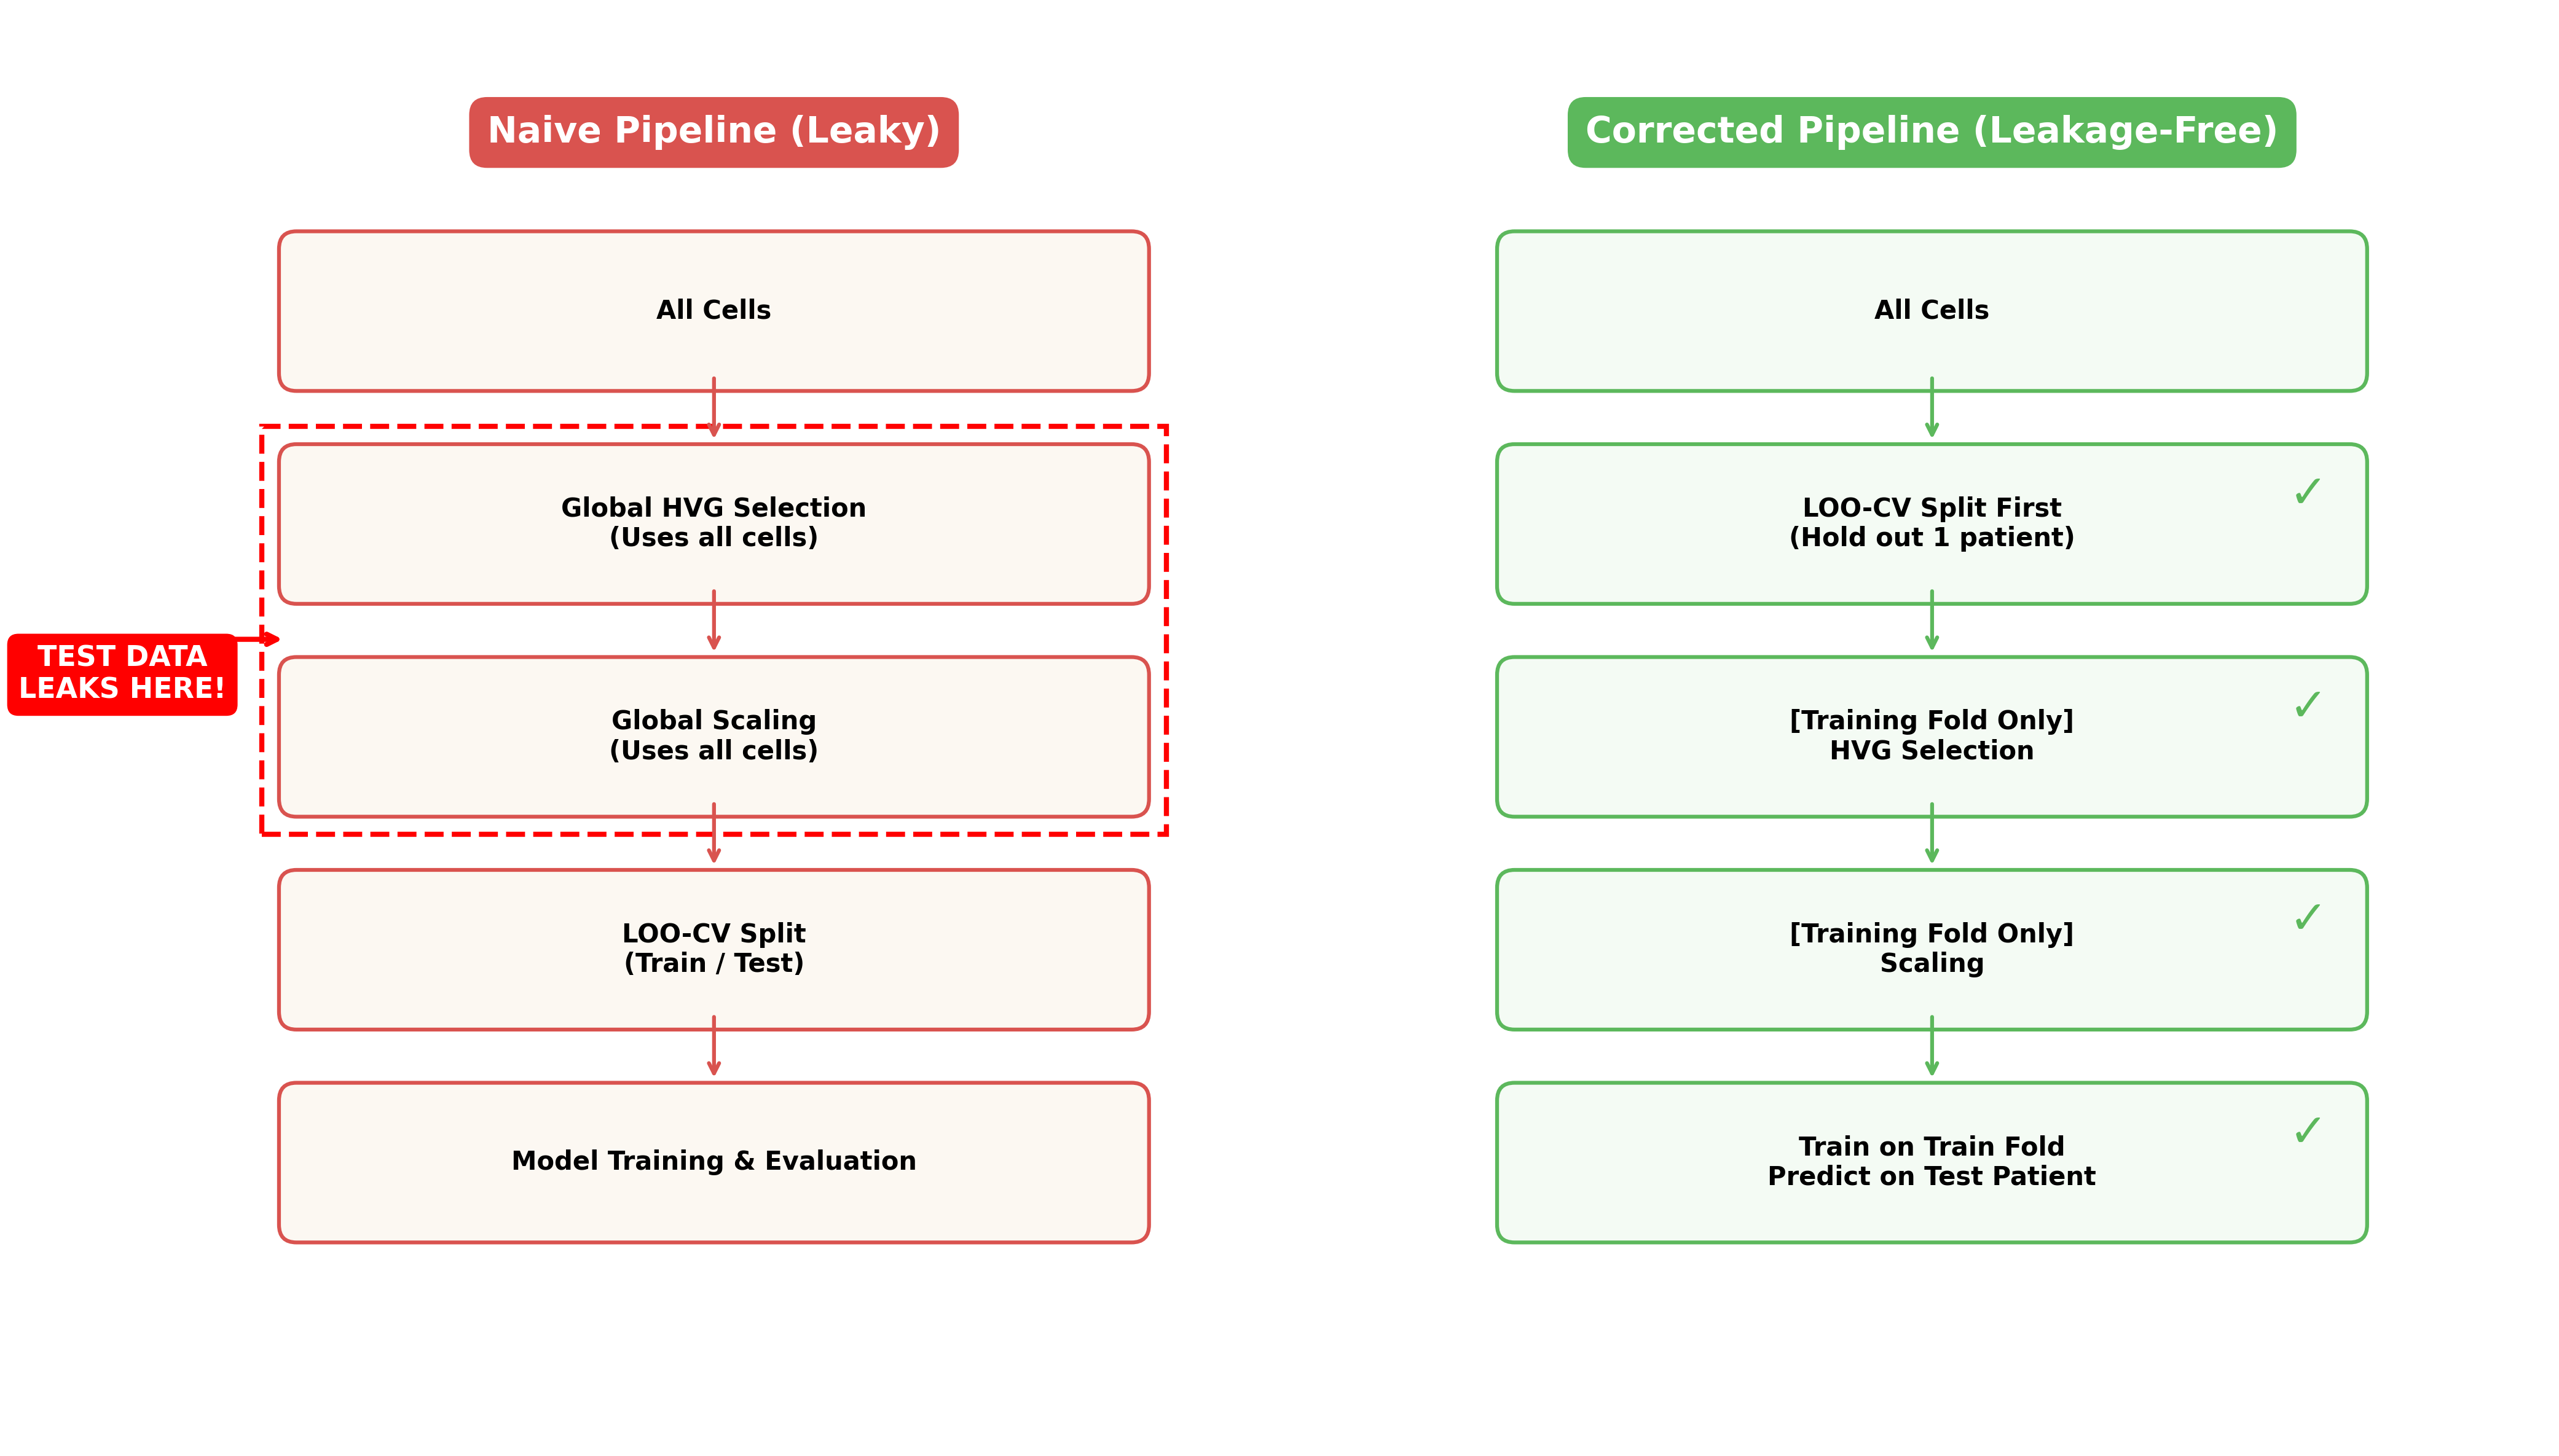
\includegraphics[width=0.98\linewidth]{figs/fig1.png}}
\caption{\csentence{Pipeline schematic comparing naive and corrected workflows.} Side-by-side comparison diagram illustrating the sources of data leakage and their correction in single-cell classification. (Left) The Naive Pipeline (Leaky) performs highly variable gene (HVG) selection and z-score scaling globally on all cells before partitioning the cross-validation splits, allowing information from the held-out test patient to leak into the training statistics. (Right) The Corrected Pipeline (Leakage-Free) performs the cross-validation split first, ensuring that all scaling and candidate feature selection steps are executed strictly within the training fold using only training patient cells.}
\label{fig:pipeline}
\end{figure}

\begin{figure}[h!]
\centerline{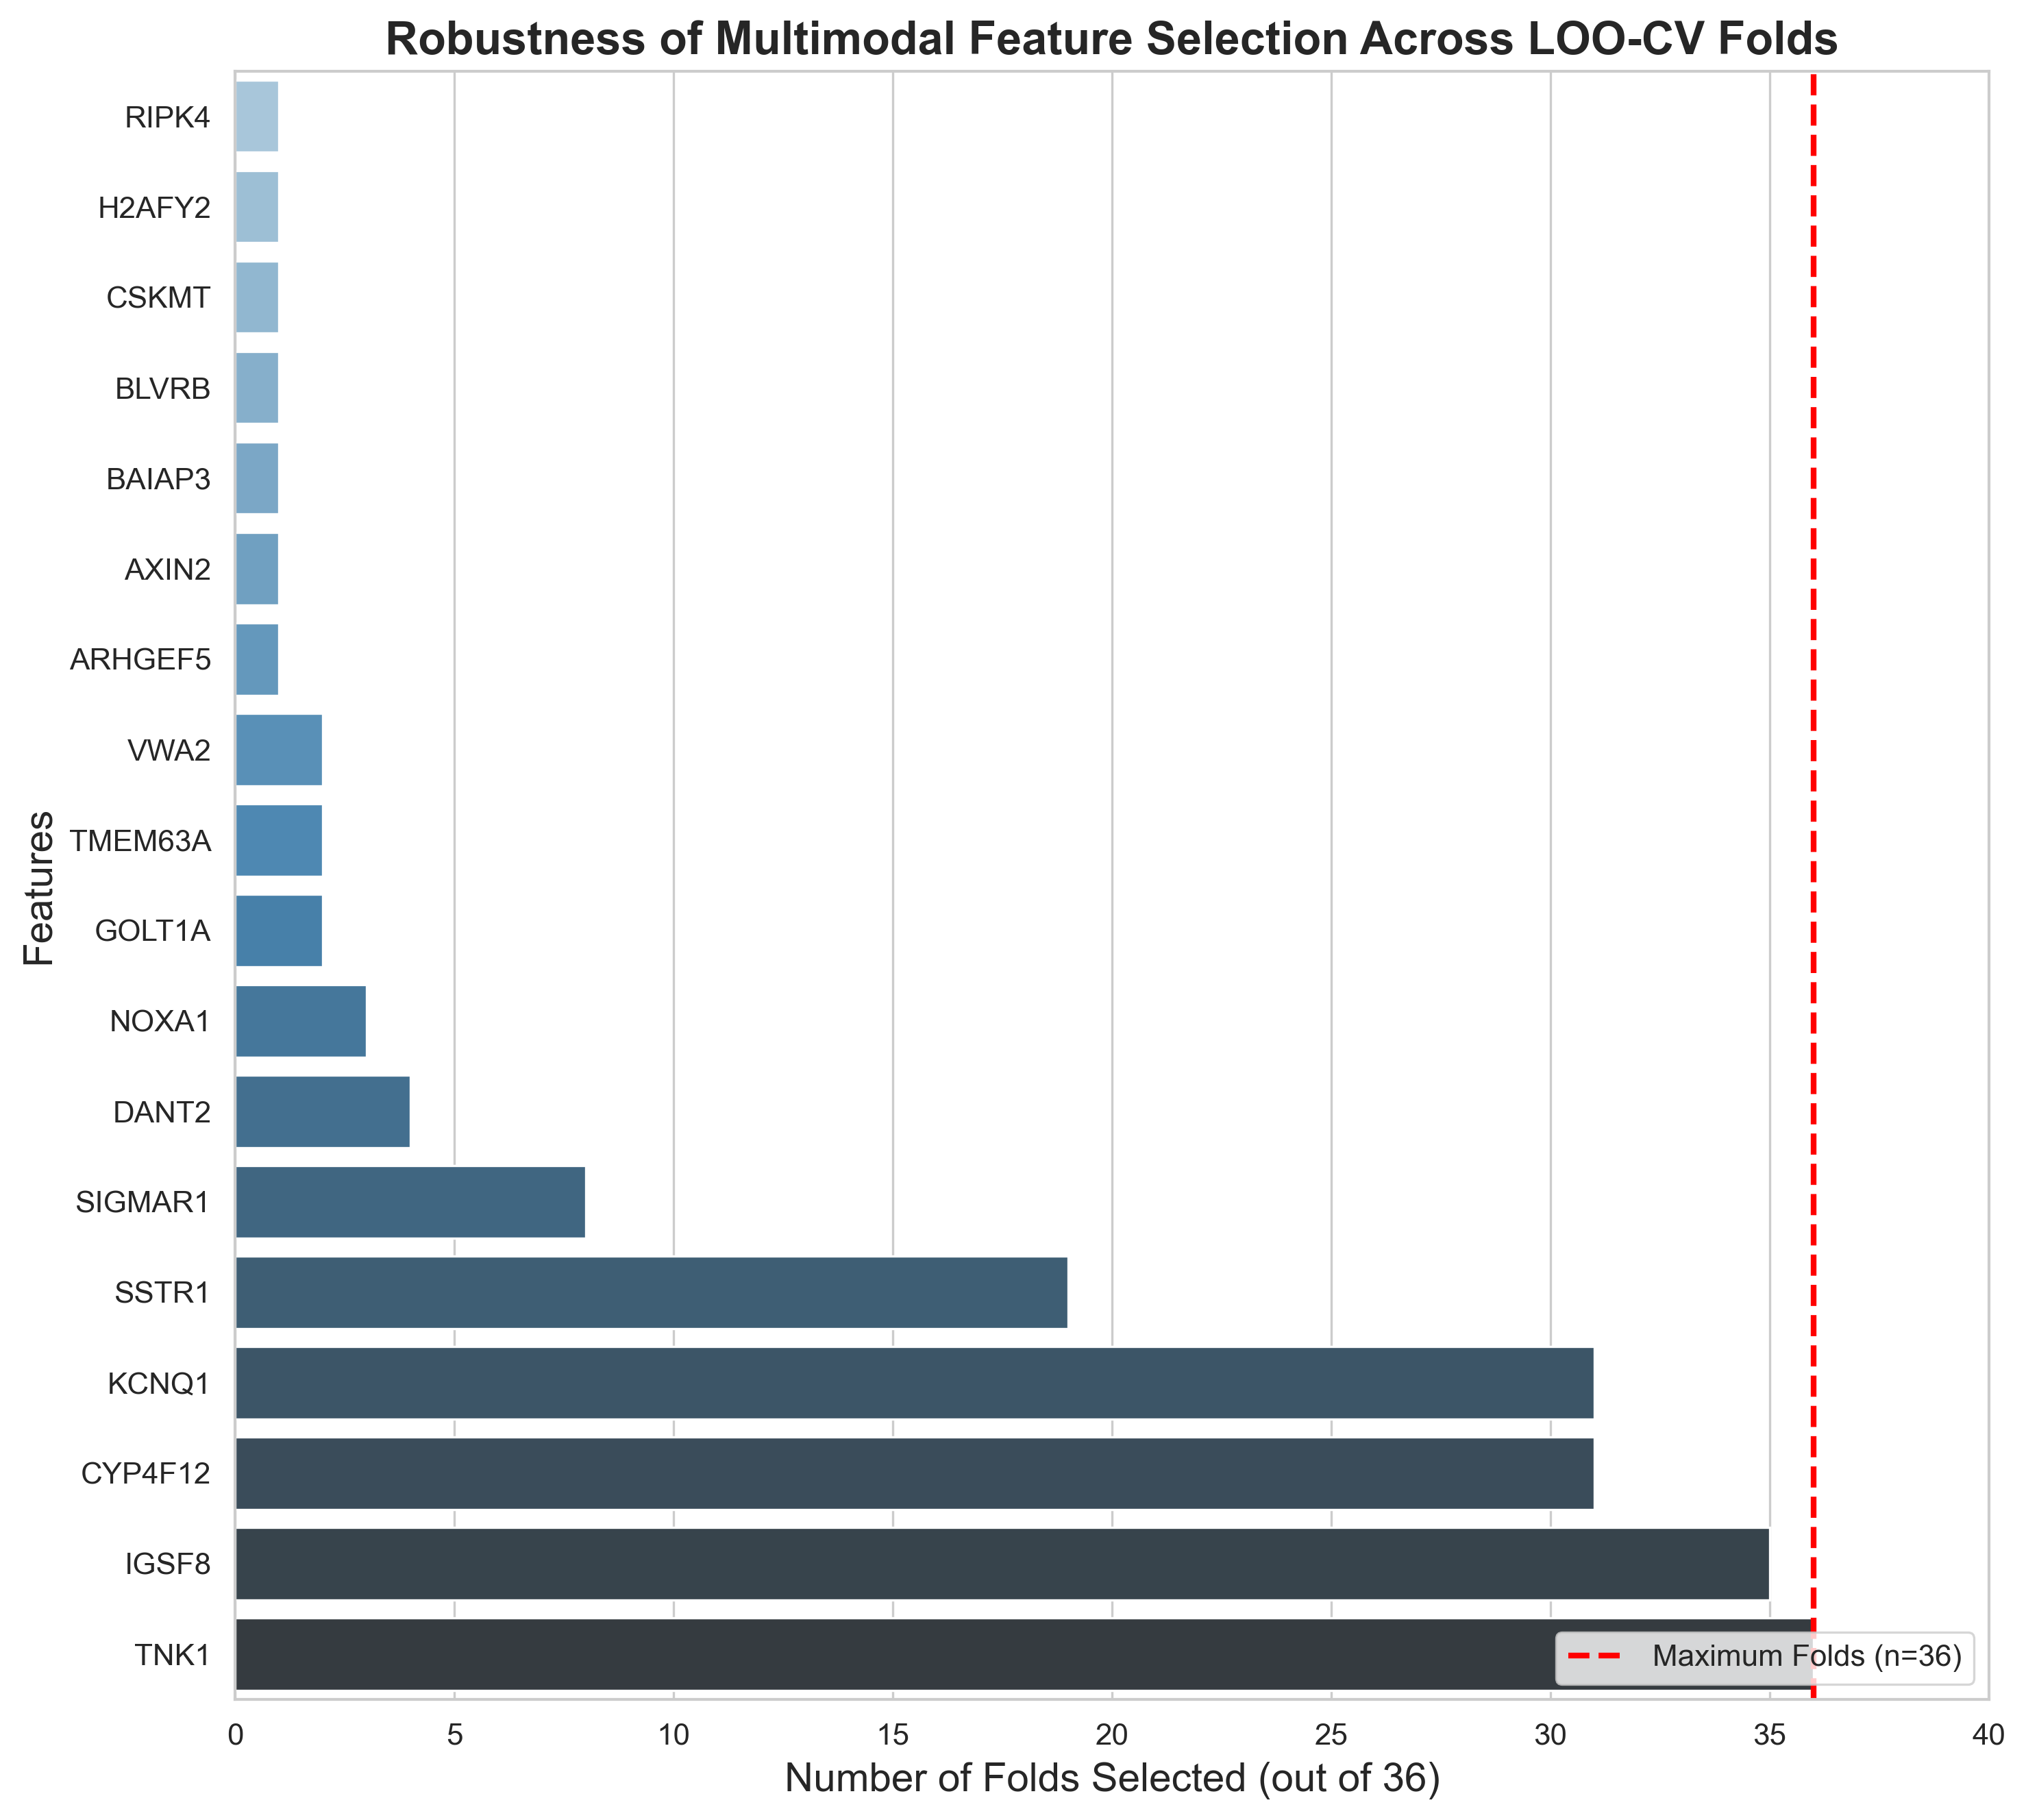
\includegraphics[width=0.98\linewidth]{figs/fig2.png}}
\caption{\csentence{Consensus feature selection frequency.} Horizontal bar chart showing all 18 features selected in at least one of the 36 Leave-One-Out Cross-Validation (LOO-CV) folds in the IBD cohort; the vertical red dashed line marks the maximum of 36 folds. \textit{TNK1} (36/36; 100.0\%) and \textit{IGSF8} (35/36; 97.2\%) were the most stable, followed by \textit{KCNQ1} and \textit{CYP4F12} (both 31/36; 86.1\%) and \textit{SSTR1} (19/36; 52.8\%); these five constitute the consensus signature, separated from the remainder by the largest gap in the distribution (19 folds to 8). The next-ranked feature, \textit{SIGMAR1}, was selected in 8/36 (22.2\%), and 10 of the 18 features were selected in 2 or fewer folds, illustrating the instability of feature selection at this cohort size.}
\label{fig:ibdstab}
\end{figure}

\begin{figure}[h!]
\centerline{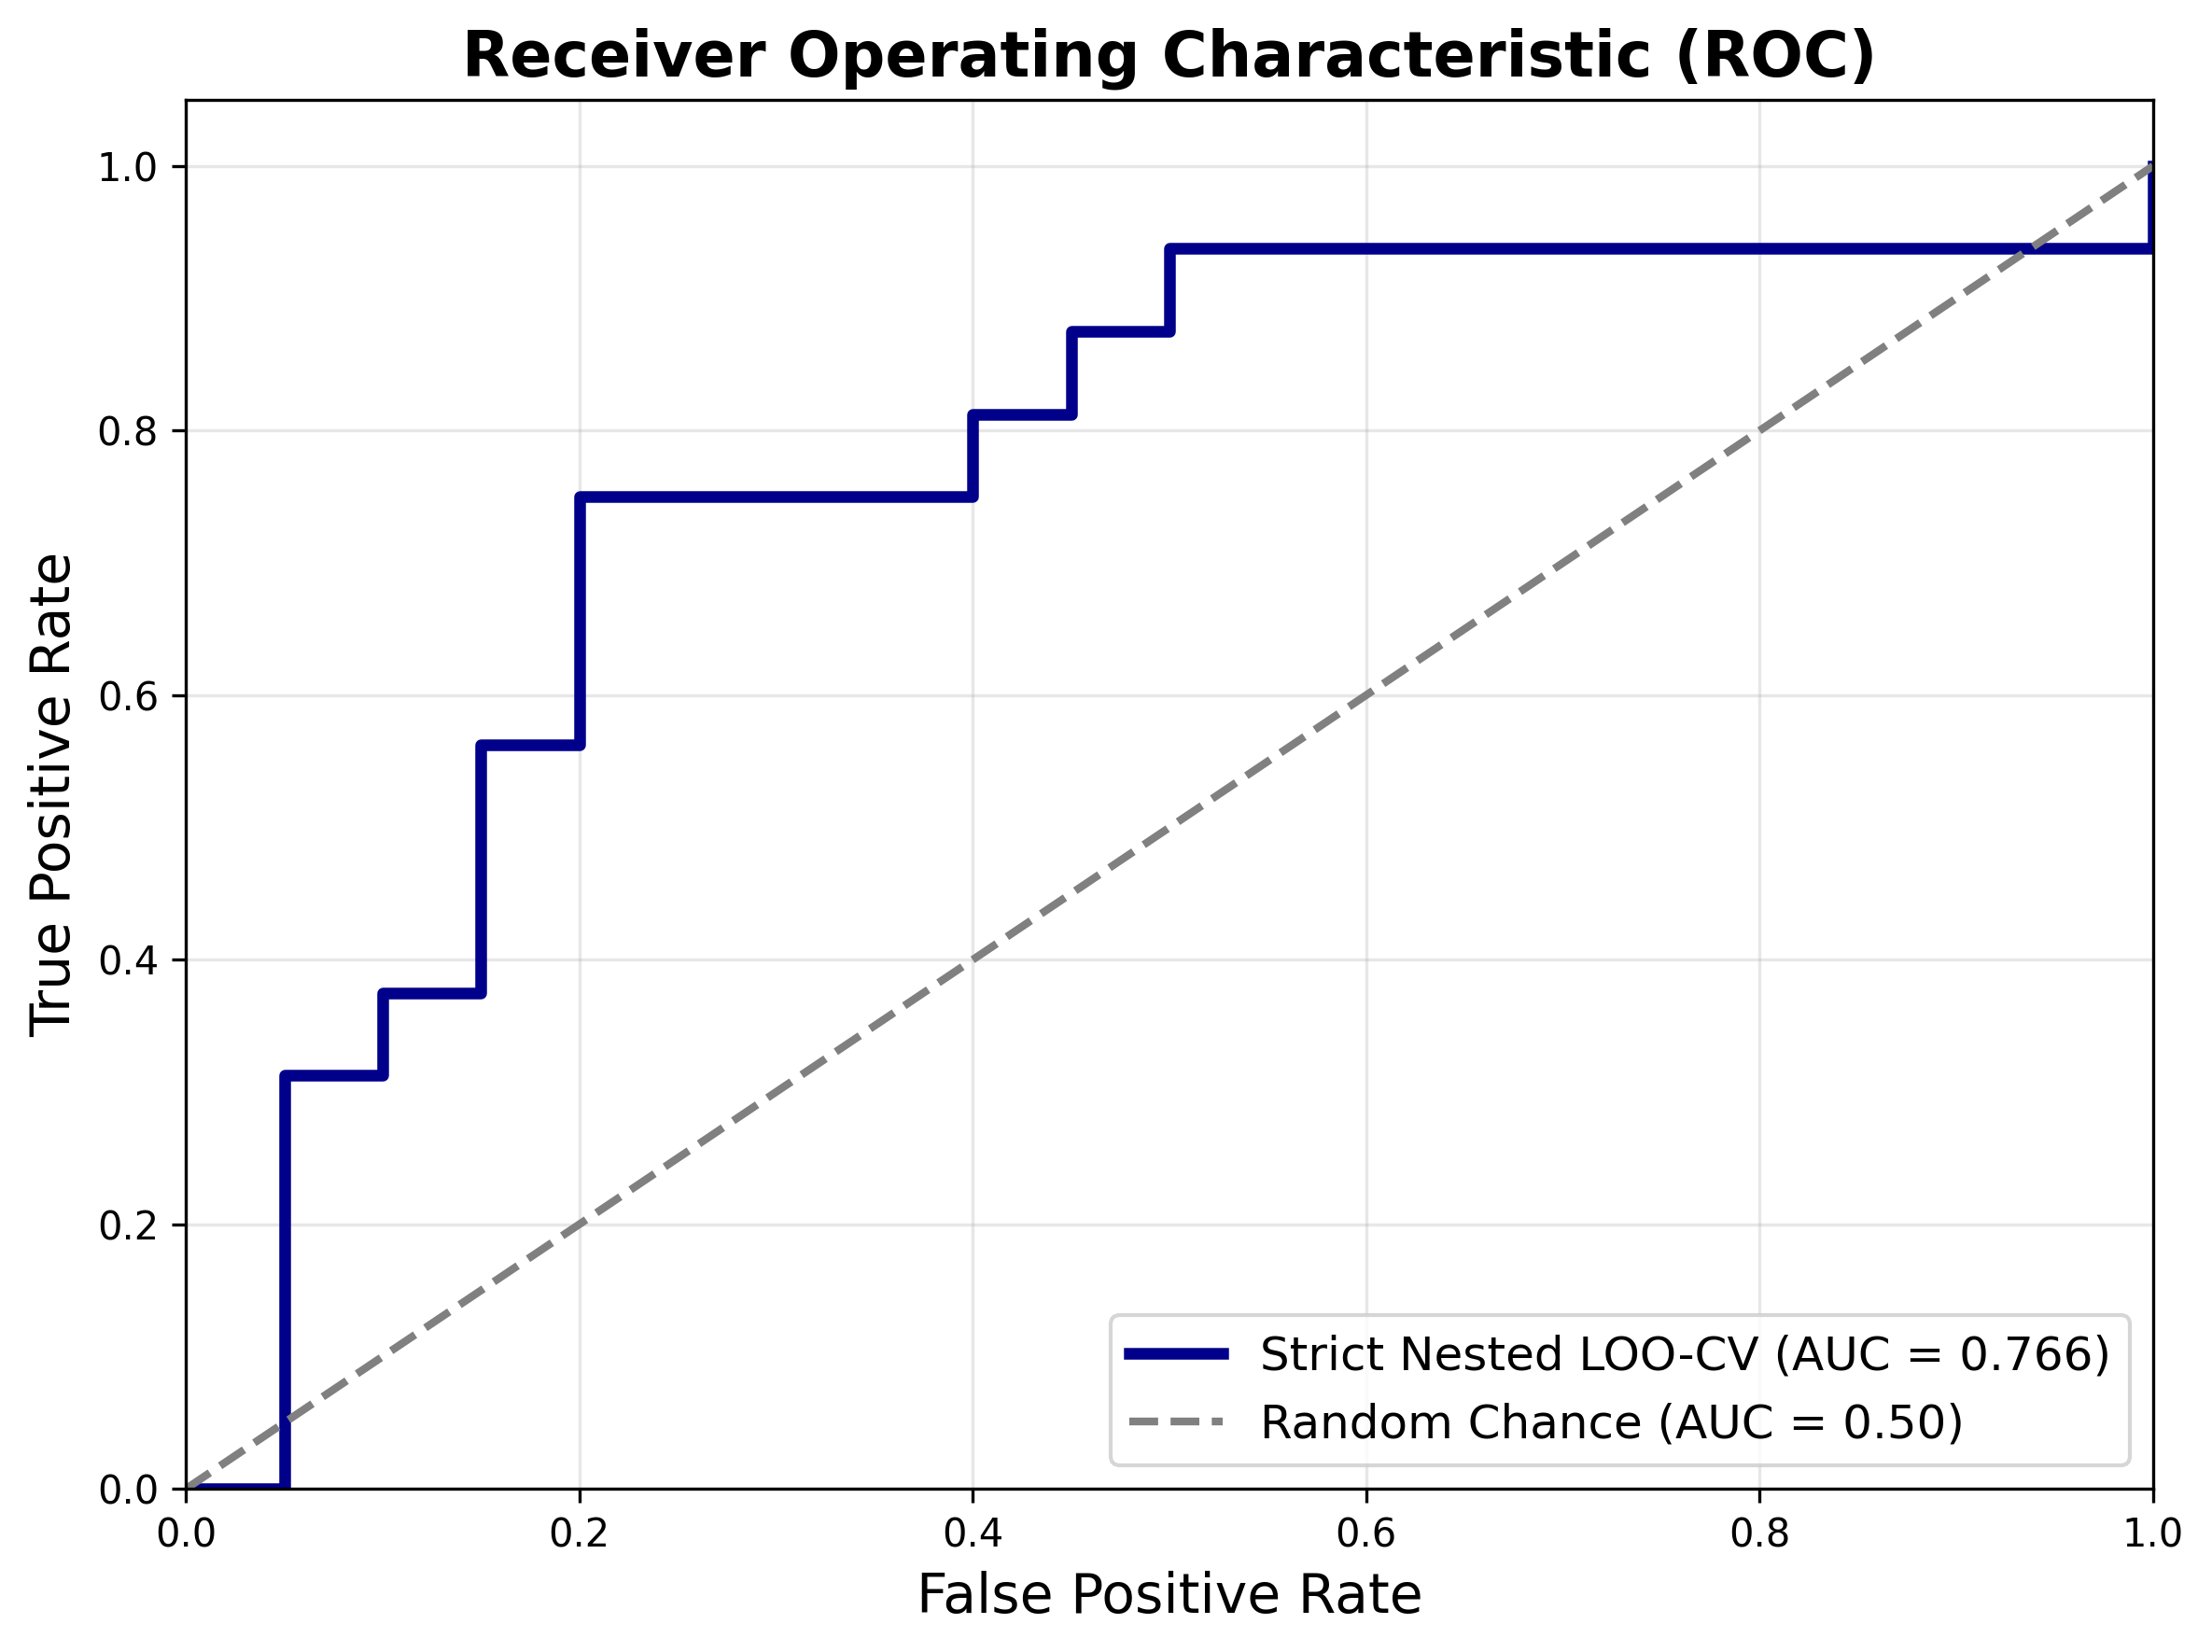
\includegraphics[width=0.98\linewidth]{figs/fig3.png}}
\caption{\csentence{Receiver Operating Characteristic (ROC) curve of the nested cross-validation model.} ROC curve representing the classification performance of the regularized Random Forest model on the IBD cohort. The solid dark blue line represents the model performance, which was evaluated by aggregating continuous prediction probabilities across the 36 independent Leave-One-Out Cross-Validation (LOO-CV) folds to maintain patient-level integrity. The diagonal gray dashed line indicates the baseline of random chance (Area Under the Curve, AUC = 0.50). The model achieved a validated AUC of 0.766, demonstrating moderate discriminative power in separating therapeutic remission from non-remission clinical outcomes.}
\label{fig:ibdroc}
\end{figure}

\begin{figure}[h!]
\centerline{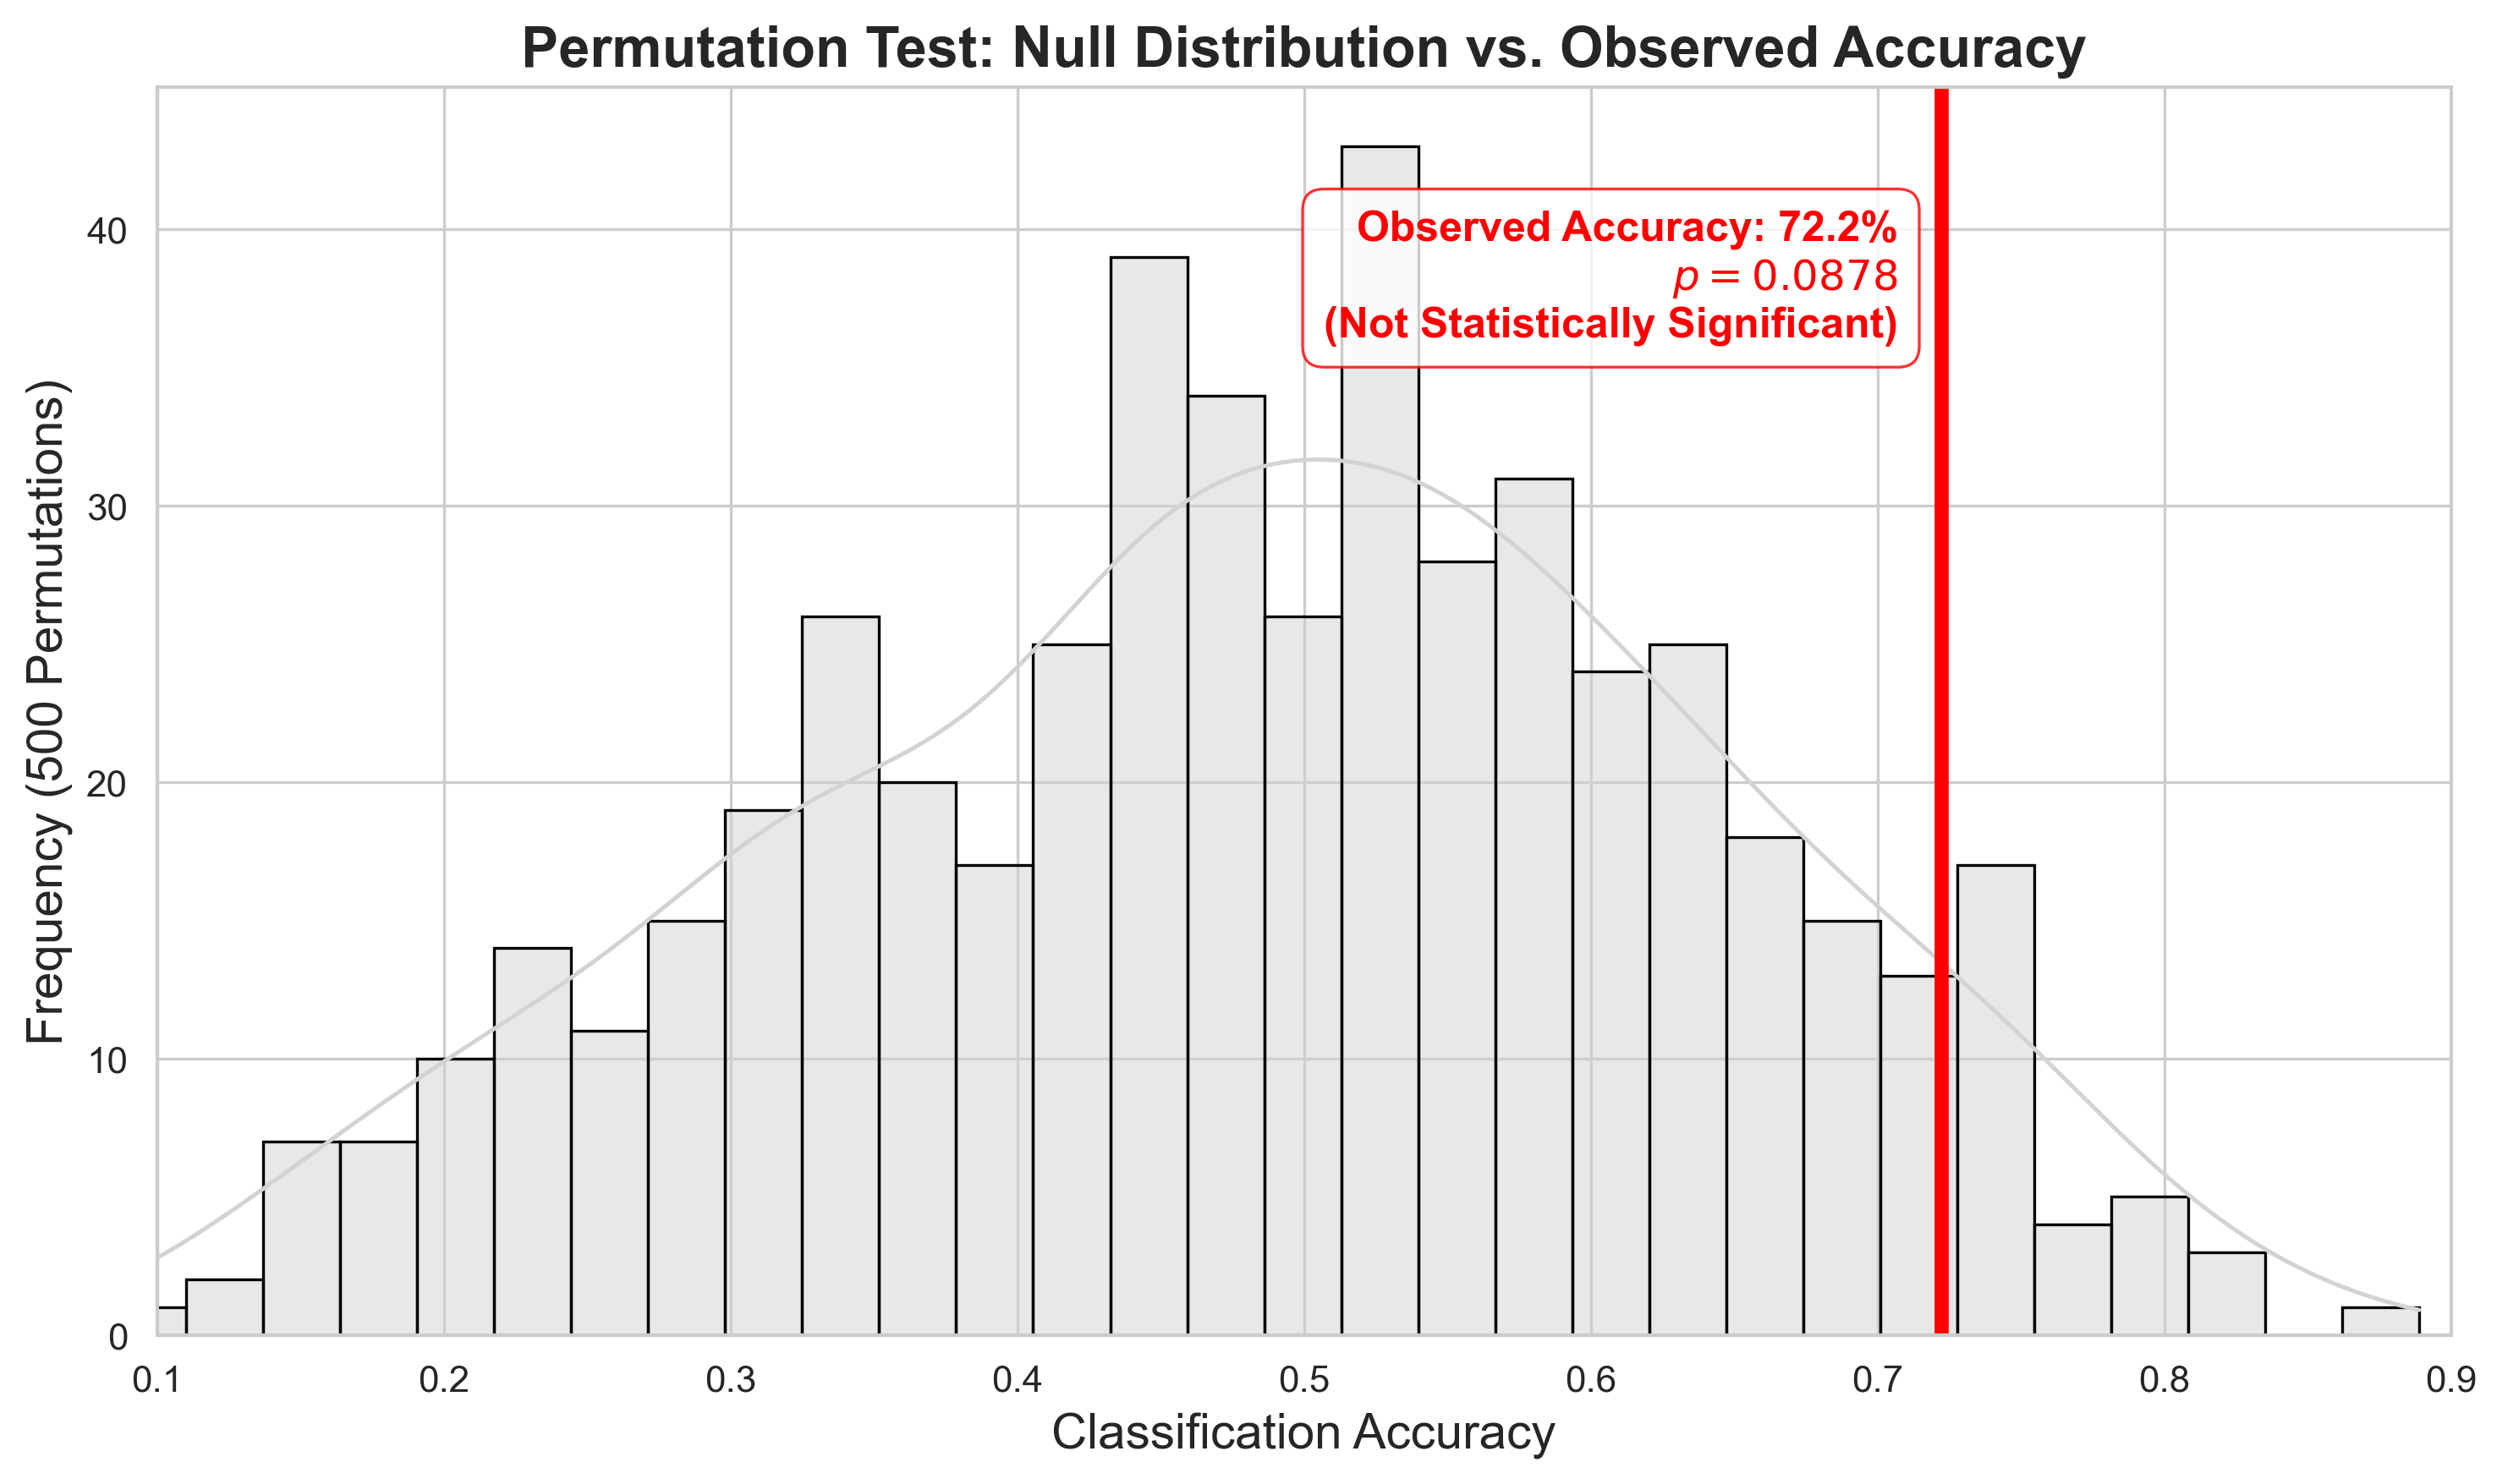
\includegraphics[width=0.98\linewidth]{figs/fig4.png}}
\caption{\csentence{Empirical null distribution generated by permutation testing.} Histogram showing the empirical null distribution of IBD classification accuracies generated from 500 iterations of label-shuffling. In each iteration, the clinical outcome labels were permuted, and the model was evaluated using the identical, strict nested Leave-One-Out Cross-Validation (LOO-CV) framework. The observed classification accuracy of the true model (72.2\%) is marked by a solid vertical red line, which did not significantly outperform the null distribution and yields an empirical significance value of $p = 0.0878$.}
\label{fig:ibdperm}
\end{figure}

\begin{figure}[h!]
\centerline{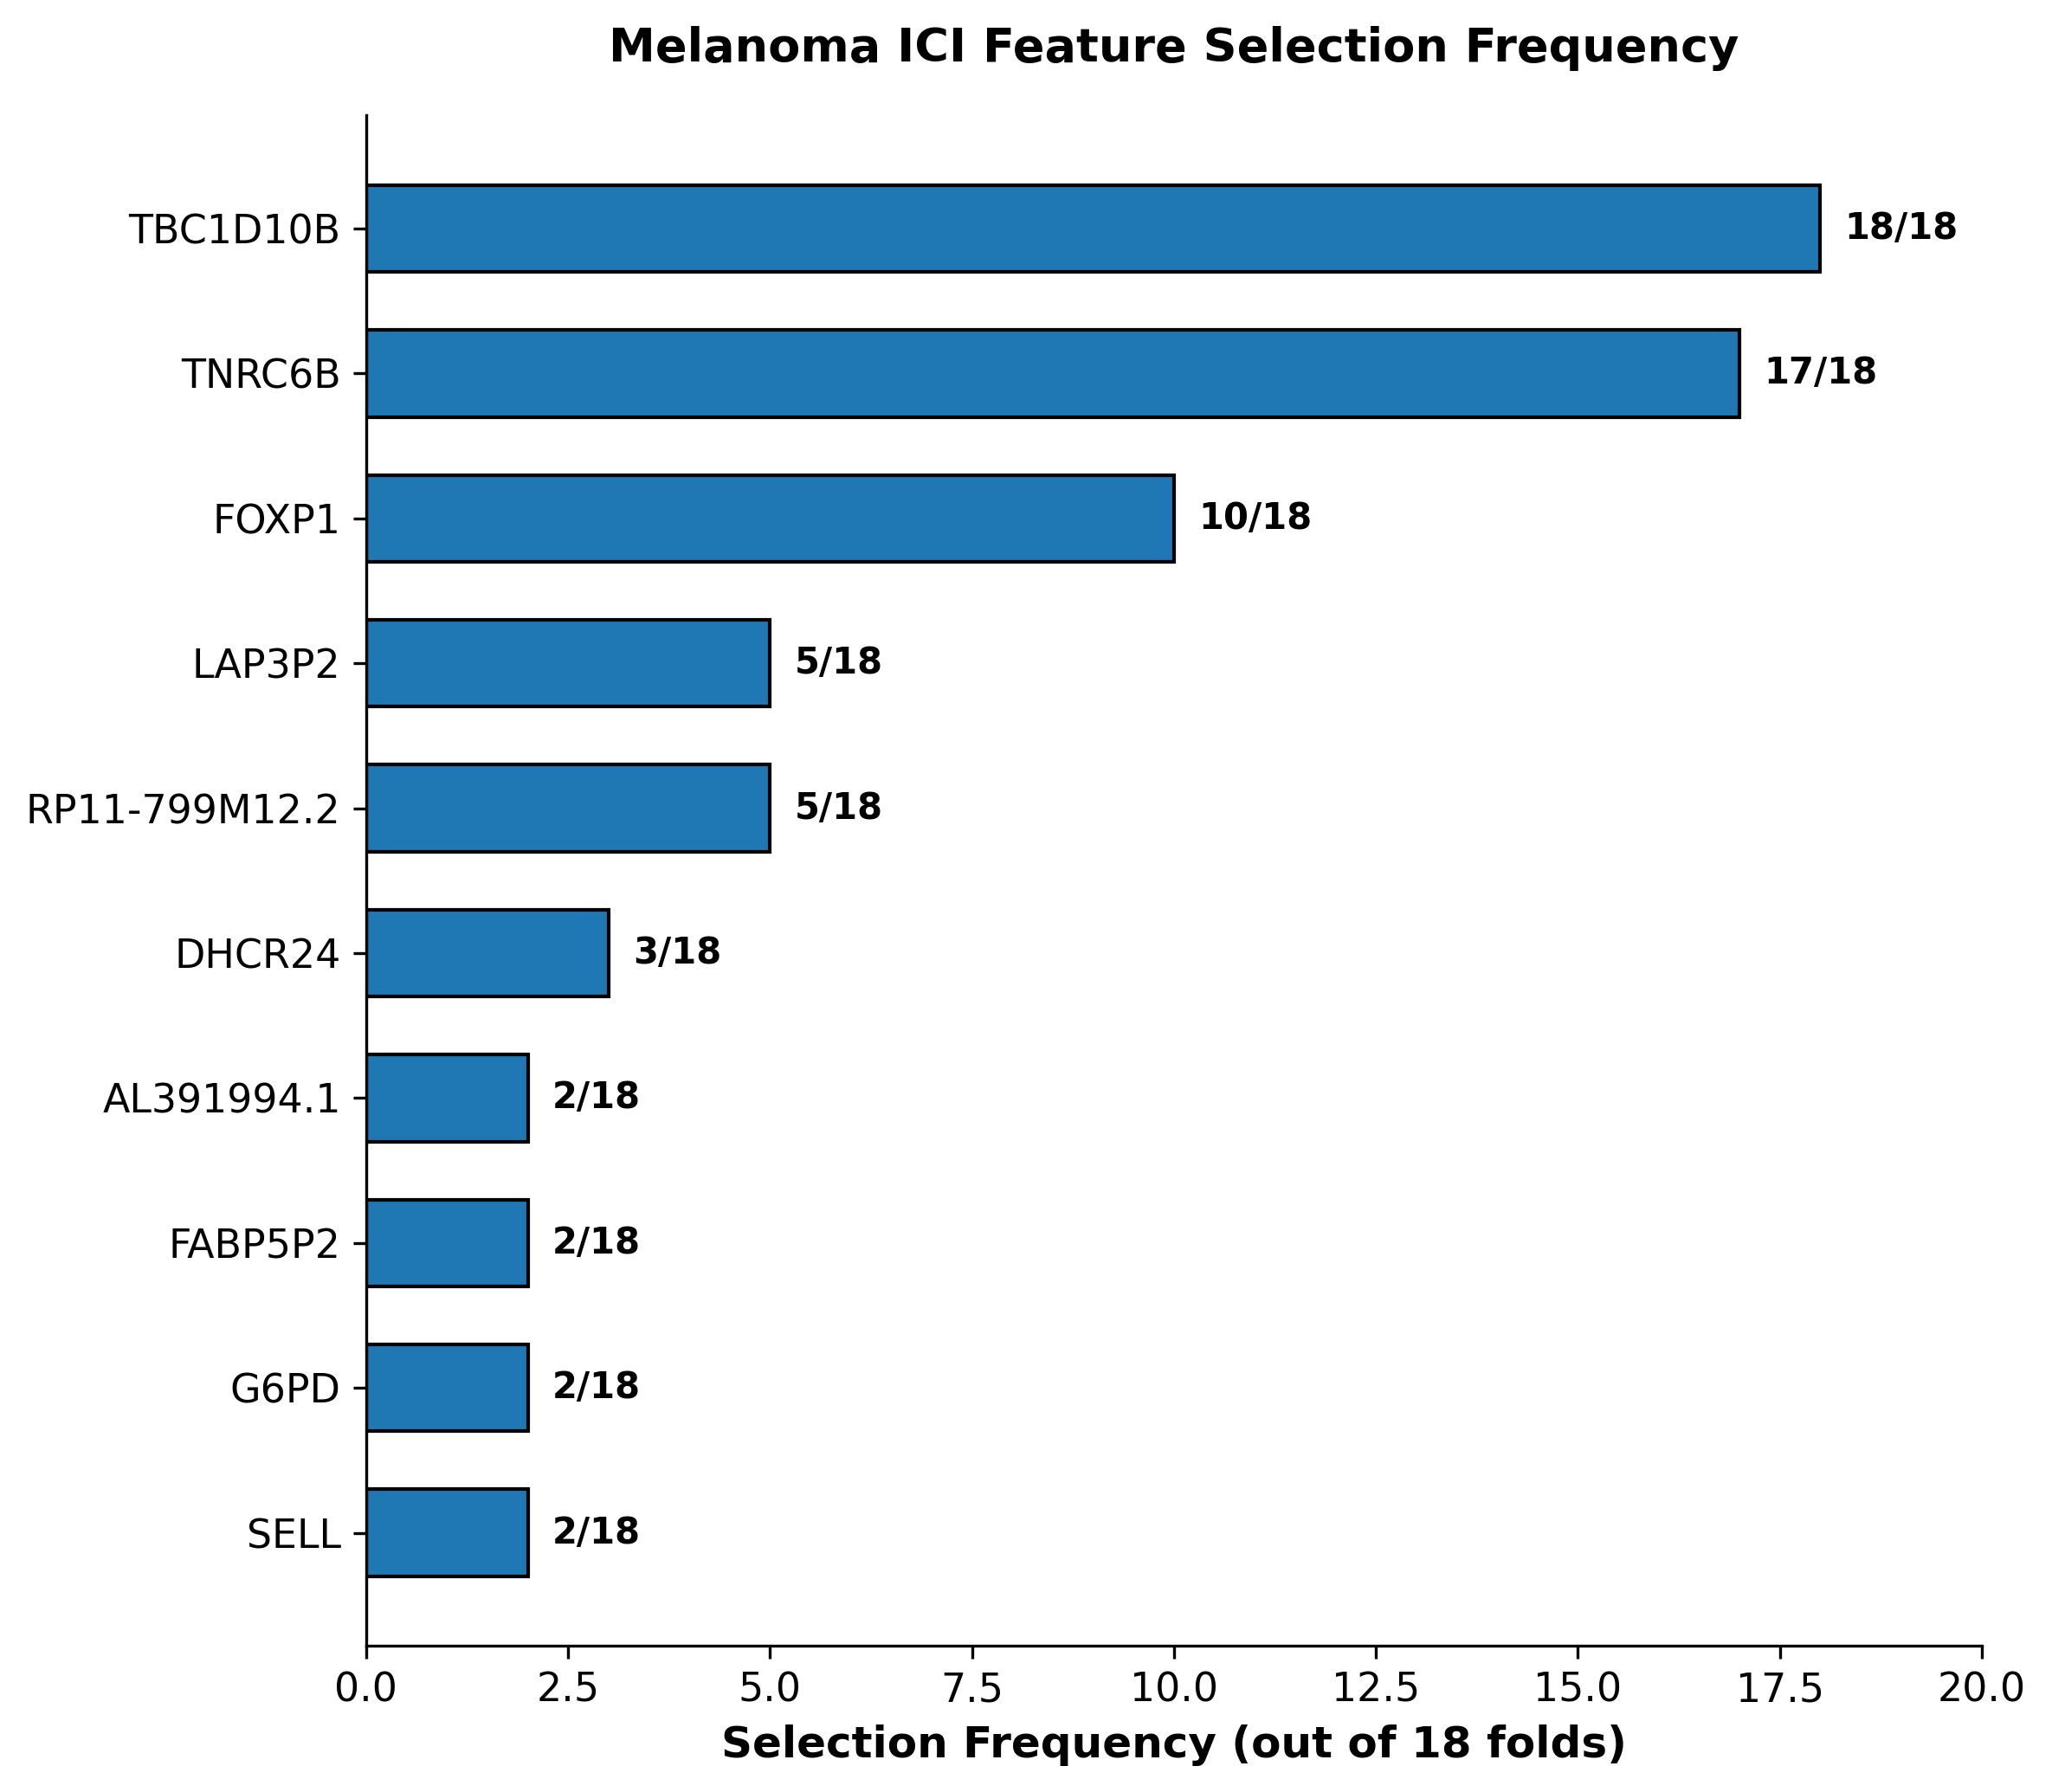
\includegraphics[width=0.98\linewidth]{figs/fig5.png}}
\caption{\csentence{Melanoma ICI feature selection frequency.} Horizontal bar chart showing selection frequency across the 18 independent Leave-One-Out Cross-Validation (LOO-CV) training folds in the melanoma cohort, for all ten genes selected in at least 2 of 18 folds: \textit{TBC1D10B} (18/18; 100.0\%), \textit{TNRC6B} (17/18; 94.4\%), \textit{FOXP1} (10), \textit{LAP3P2} (5), \textit{RP11-799M12.2} (5), \textit{DHCR24} (3), and \textit{AL391994.1}, \textit{FABP5P2}, \textit{G6PD} and \textit{SELL} (2 each). A further 24 genes were selected in exactly one fold, for 34 in total. Per-fold frequencies for all 34 genes are provided in the accompanying repository.}
\label{fig:melstab}
\end{figure}

\begin{figure}[h!]
\centerline{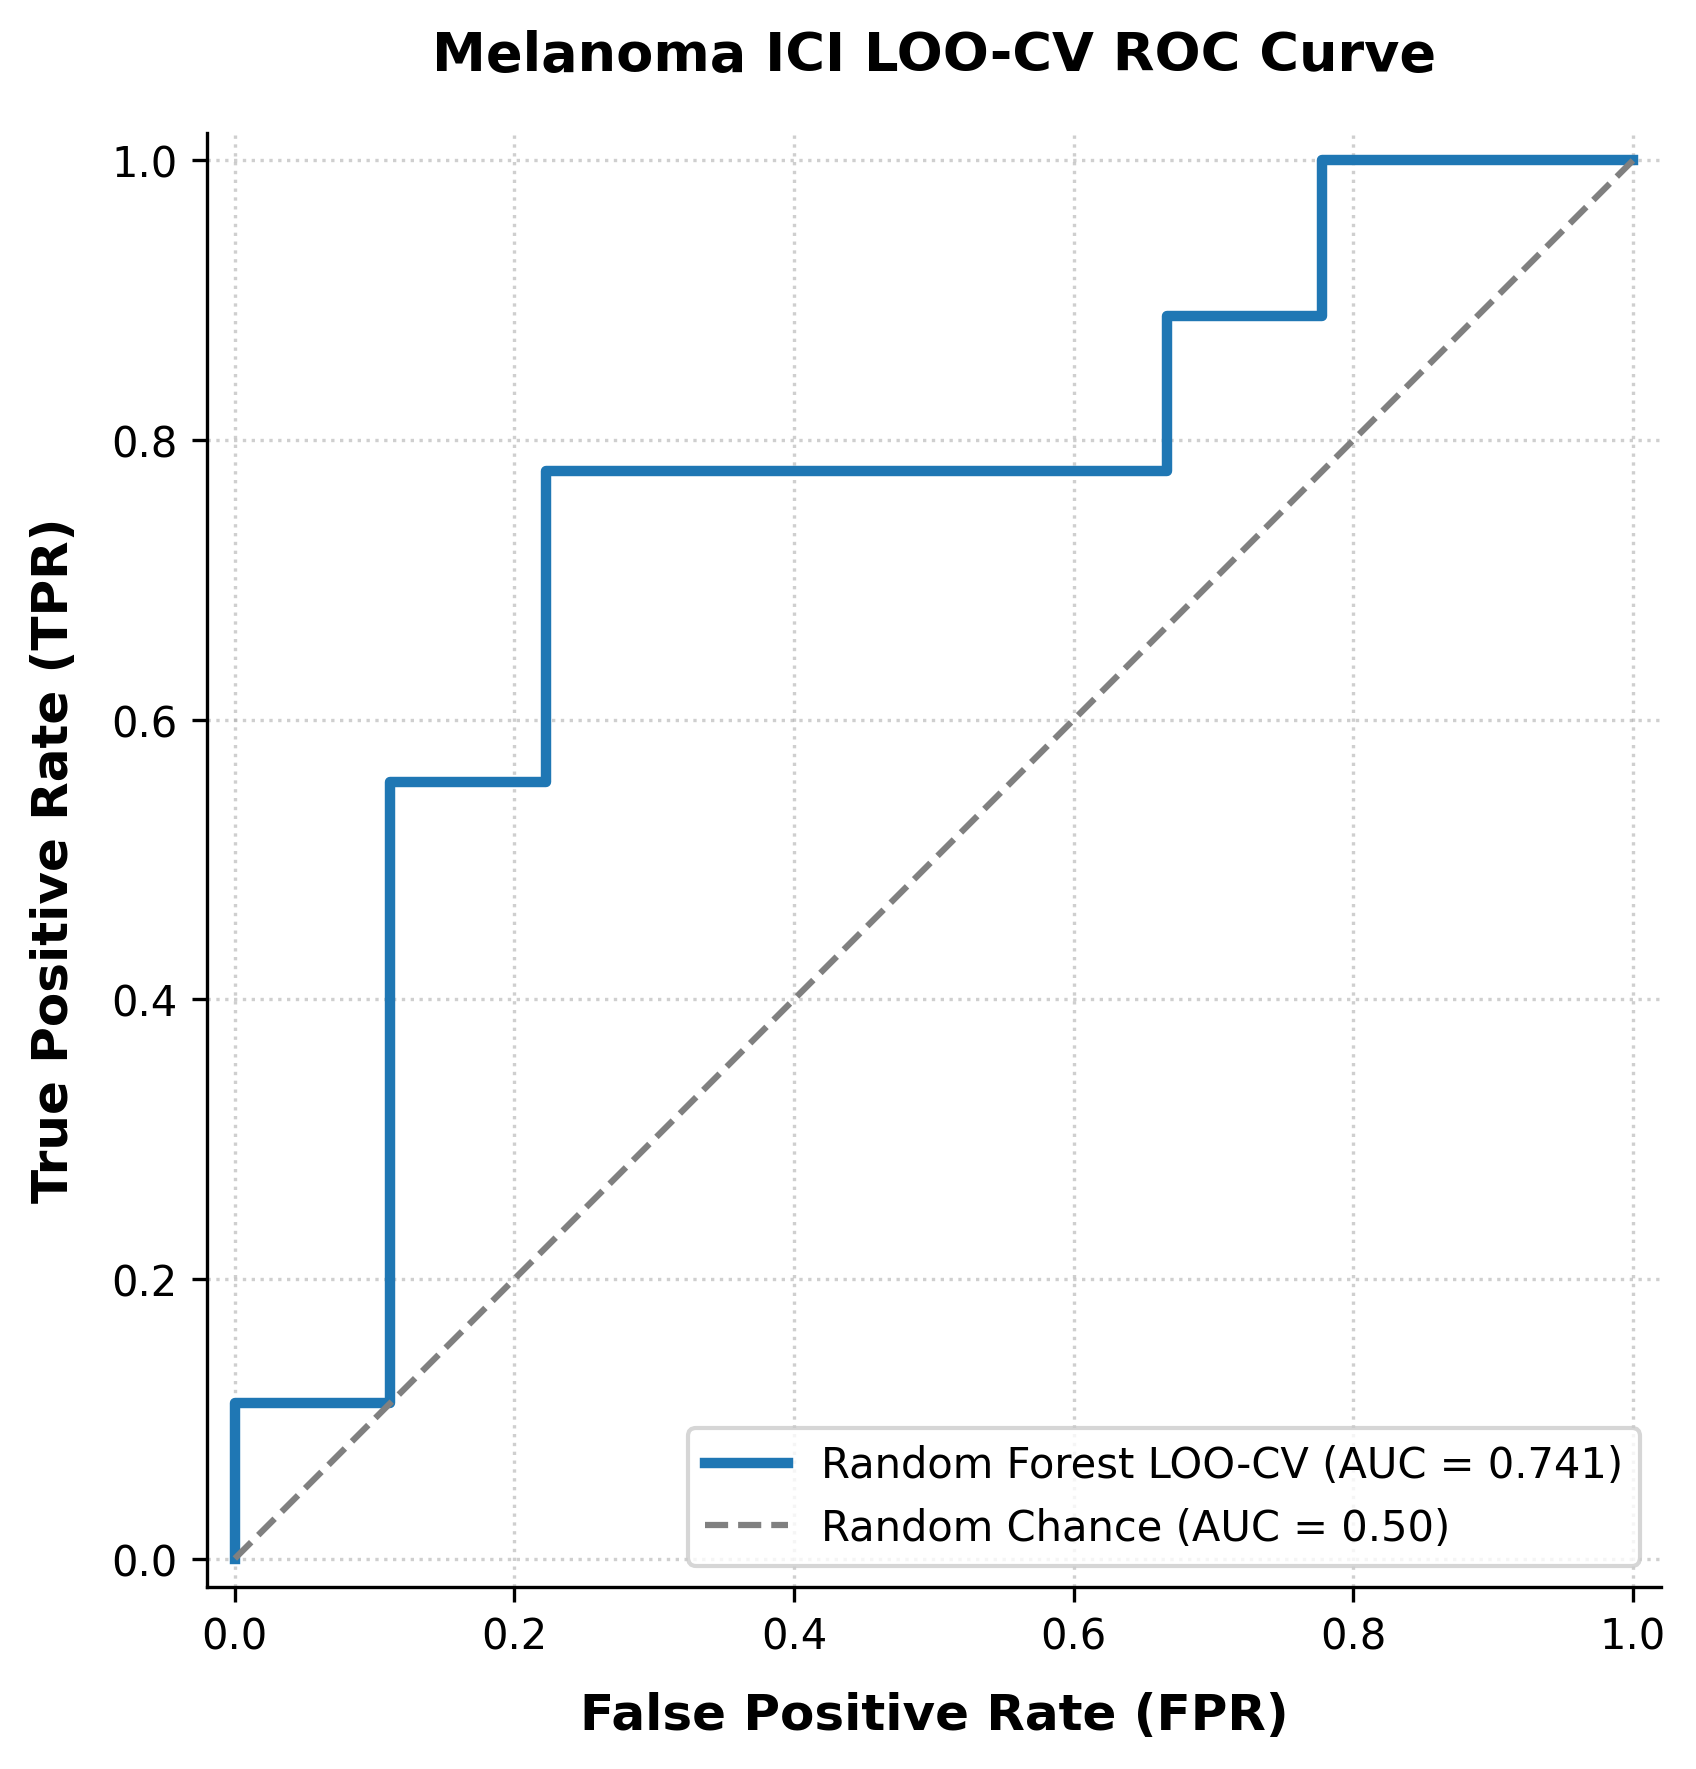
\includegraphics[width=0.98\linewidth]{figs/fig6.png}}
\caption{\csentence{Receiver Operating Characteristic (ROC) curve of the melanoma ICI cross-validation model.} ROC curve representing the classification performance of the regularized Random Forest model on the melanoma dataset. The solid dark blue line represents the model performance evaluated by aggregating prediction probabilities across the 18 independent Leave-One-Out Cross-Validation (LOO-CV) folds. The diagonal gray dashed line indicates the baseline of random chance (AUC = 0.50). The model achieved a validated AUC of 0.741, indicating moderate out-of-sample discriminative capacity.}
\label{fig:melroc}
\end{figure}

\end{backmatter}
\end{document}
